% !TEX root = ../main.tex
\chapter{Bloch 定理与二维光子晶体基础}
\label{ch:bloch}

\section*{学习目标}
\begin{itemize}
  \item 理解平移对称性为什么会导致 Bloch 定理，而不只是记住 Bloch 形式。
  \item 掌握二维晶格、倒晶格、布里渊区和高对称点的基本几何意义。
  \item 认识 slab 结构中 TE/TM 分类的适用条件与局限。
\end{itemize}

\section*{先修知识}
\cref{ch:maxwell,ch:roadmap} 中的频域 Maxwell 方程、坐标约定和倒格矢记号。

\section*{本章路线图}
\ChapterModelLevel{L1}
本章先从“周期性如何约束解”讲起，再给出 Bloch 定理的证明思路，随后介绍二维光子晶体几何和布里渊区，最后把这些理想周期概念放回具有有限厚度的 PCSEL slab 结构中，解释 TE/TM 为什么经常只是近似语言。

\section{为什么周期性如此重要}
上一章已经说明，PCSEL 的被动光学问题来自开放系统中的 Maxwell 方程。现在我们加入新的结构信息：介电函数在平面内是周期的。设存在一组晶格平移 $\bm{R}$，使得
\begin{equation}
\varepsilon(\rho+\bm{R},z)=\varepsilon(\rho,z).
\label{eq:lattice_periodicity}
\end{equation}
这条看似普通的式子，带来的影响极大。它意味着：虽然结构在平面上无限延展，但解并不需要在整个无限空间里“毫无组织地”寻找。周期性会把解空间分解成一族由波矢 $\kvec$ 标记的子空间。Bloch 定理正是这种分解的数学表达。

对初学者来说，Bloch 定理最容易被误记成一句形式化定义
\[
\E_{\kvec}(\rvec)=\ee^{\ii\kvec\cdot\rho}\bm{u}_{\kvec}(\rvec),
\]
然后就往下继续算。这样当然可以做题，但很难真正理解为什么这一形式自然、为什么它和倒格矢、高对称点、能带图联系如此紧密。要把后面的 PCSEL 模分析学扎实，最好先从“对称算符”角度理解这件事。

\section{Bloch 定理的来源：平移算符与共同本征态}
考虑晶格平移算符 $\hat T_{\bm{R}}$，定义为
\[
\hat T_{\bm{R}}\E(\rho,z)=\E(\rho+\bm{R},z).
\]
若介质满足 \cref{eq:lattice_periodicity}，则 Maxwell 算符在平面内与所有 $\hat T_{\bm{R}}$ 对易。这一点最好显式写一次。设频域算子记为
\[
\hat{\mathcal L}
=
\nabla\times \mu_r^{-1}(\rho,z)\nabla\times
-\frac{\omega^2}{c^2}\varepsilon_r(\rho,z),
\]
则对任意场 $\E$ 有
\[
\hat T_{\bm R}\hat{\mathcal L}\E(\rho,z)
=
\hat{\mathcal L}(\rho+\bm R,z)\E(\rho+\bm R,z).
\]
一旦结构满足
\[
\varepsilon_r(\rho+\bm R,z)=\varepsilon_r(\rho,z),
\qquad
\mu_r(\rho+\bm R,z)=\mu_r(\rho,z),
\]
就有 $\hat{\mathcal L}(\rho+\bm R,z)=\hat{\mathcal L}(\rho,z)$，从而
\[
\hat T_{\bm R}\hat{\mathcal L}\E
=
\hat{\mathcal L}\hat T_{\bm R}\E,
\qquad\Longrightarrow\qquad
[\hat T_{\bm R},\hat{\mathcal L}]=0.
\]
对易意味着可以寻找同时是 Maxwell 算符和平移算符本征态的场。于是存在一组复数 $\lambda(\bm{R})$ 使得
\[
\hat T_{\bm{R}}\E(\rho,z)=\lambda(\bm{R})\E(\rho,z).
\]

现在利用群性质：
\[
\hat T_{\bm{R}_1}\hat T_{\bm{R}_2}=\hat T_{\bm{R}_1+\bm{R}_2}.
\]
对同一本征态作用后得到
\[
\lambda(\bm{R}_1)\lambda(\bm{R}_2)=\lambda(\bm{R}_1+\bm{R}_2).
\]
满足这种可乘性质的连续表示只能写成
\[
\lambda(\bm{R})=\ee^{\ii\kvec\cdot\bm{R}},
\]
其中 $\kvec$ 是某个二维向量。一个简要论证如下：若 $\lambda(\bm{R})$ 连续且满足 $\lambda(\bm{R}_1)\lambda(\bm{R}_2)=\lambda(\bm{R}_1+\bm{R}_2)$，则可写 $\ln\lambda(\bm{R})=\bm{c}\cdot\bm{R}$，其中 $\bm{c}$ 为常向量。无损周期系统要求 $|\lambda|=1$，因此 $\bm{c}$ 必为纯虚数，记作 $\ii\kvec$，于是得到指数形式。若允许有损或倏逝 Bloch 解，则 $\kvec$ 可取复数（“复 Bloch 波矢”），对应沿晶格方向的衰减或放大。

于是便有
\begin{equation}
\E_{\kvec}(\rho+\bm{R},z)=\ee^{\ii\kvec\cdot\bm{R}}\E_{\kvec}(\rho,z),
\label{eq:bloch_condition}
\end{equation}
再把快速相位因子提出，就得到Bloch 形式
\begin{equation}
\E_{\kvec}(\rho,z)=\ee^{\ii\kvec\cdot\rho}\bm{u}_{\kvec}(\rho,z),
\qquad
\bm{u}_{\kvec}(\rho+\bm{R},z)=\bm{u}_{\kvec}(\rho,z).
\label{eq:bloch_form}
\end{equation}

\begin{figure}[htbp]
  \centering
  % !TEX root = ../main.tex
% Figure content only: inserted inside an outer figure environment in ch04
\begin{tikzpicture}[x=0.92cm,y=0.92cm]
  \tikzset{
    paneltitle/.style={font=\bfseries},
    infobox/.style={draw,rounded corners,thick,fill=blue!5,align=center}
  }

  \begin{scope}[xshift=-4.7cm]
    \node[paneltitle] at (0,2.1) {(a) 周期系数};
    \draw[->,thick] (-2.8,0) -- (2.8,0) node[right] {$x$};
    \draw[->,thick] (-2.8,-1.0) -- (-2.8,1.8) node[above] {$V(x)$};
    \draw[blue!70,thick,domain=-2.6:2.6,samples=140] plot(\x,{0.8+0.55*cos(\x r*2)});
    \draw[dashed,gray] (-1.57,0) -- (-1.57,1.5);
    \draw[dashed,gray] (1.57,0) -- (1.57,1.5);
    \draw[<->,thick] (-1.57,1.35) -- (1.57,1.35) node[midway,above,font=\scriptsize] {$a$};
    \node[font=\scriptsize,blue!70] at (1.2,0.45) {$V(x+a)=V(x)$};
  \end{scope}

  \begin{scope}[xshift=0cm]
    \node[paneltitle] at (0,2.1) {(b) Bloch 形式};
    \draw[->,thick] (-2.8,0) -- (2.8,0) node[right] {$x$};
    \draw[->,thick] (-2.8,-1.6) -- (-2.8,1.8) node[above] {$\psi_k(x)$};
    \draw[blue!70,dashed,thick,domain=-2.6:2.6,samples=140] plot(\x,{0.65*cos(\x r)});
    \draw[red!70,dotted,thick,domain=-2.6:2.6,samples=180] plot(\x,{0.30*sin(3*\x r)});
    \draw[green!50!black,thick,domain=-2.6:2.6,samples=180] plot(\x,{0.52*cos(\x r)+0.18*sin(3*\x r)});
    \node[font=\scriptsize,blue!70] at (-1.2,1.0) {$u_k(x)$};
    \node[font=\scriptsize,red!70] at (1.1,-1.0) {$\ee^{\ii kx}$};
    \node[font=\scriptsize,green!50!black,align=center] at (1.0,1.35) {$\psi_k=u_k\,\ee^{\ii kx}$};
  \end{scope}

  \begin{scope}[xshift=4.8cm]
    \node[paneltitle] at (0,2.1) {(c) 与光子晶体类比};
    \draw[thick] (-2.2,1.4) rectangle (2.2,-1.3);
    \draw[thick] (0,1.4) -- (0,-1.3);
    \draw[thick] (-2.2,0.7) -- (2.2,0.7);
    \draw[thick] (-2.2,-0.1) -- (2.2,-0.1);
    \node[font=\scriptsize] at (-1.1,1.05) {系统};
    \node[font=\scriptsize] at (1.1,1.05) {控制方程};
    \node[font=\scriptsize] at (-1.1,0.30) {电子};
    \node[font=\tiny,align=center,text width=1.9cm] at (1.1,0.30)
      {$[-\nabla^2+V]\psi=E\psi$};
    \node[font=\scriptsize] at (-1.1,-0.50) {光子};
    \node[font=\tiny,align=center,text width=1.9cm] at (1.1,-0.50)
      {$[\nabla\times\nabla\times-\frac{\omega^2}{c^2}\epsilon]\mathbf{H}=0$};
    \node[font=\scriptsize,align=center,text width=3.8cm] at (0,-0.95)
      {共同点：周期系数、平移对称、均满足 Bloch 定理};
  \end{scope}

  \node[infobox,font=\small,text width=12.2cm] at (0,-3.2) {
    \textbf{Bloch 定理：}
    周期系统中的本征解可写为
    $\psi_{\bm{k}}(\bm{r}) = u_{\bm{k}}(\bm{r})\,\ee^{\ii \bm{k}\cdot \bm{r}}$，
    其中 $u_{\bm{k}}(\bm{r}+\bm{R}) = u_{\bm{k}}(\bm{r})$ 与晶格同周期。
  };
\end{tikzpicture}

  \caption{一维 Bloch定理直观演示。(a)周期势场$V(x)$（黑色）与 Bloch波函数$|\psi_k(x)|^2$（彩色）；(b) Bloch波函数的分解：包络函数$|u_k(x)|^2$（红色虚线，具有与晶格相同的周期性）乘以平面波因子（蓝色振荡）；(c) 电子系统与光子系统的类比：尽管控制方程不同（Schrödinger 方程vs Maxwell 方程），但由于两者都是线性波动方程且具有周期系数，Bloch 定理的数学形式完全相同。这使得我们可以将固体物理中的能带理论直接迁移到光子晶体。}
  \label{fig:ch04_bloch_1d_demo}
\end{figure}

\cref{fig:ch04_bloch_1d_demo}通过一维示例直观展示了Bloch 定理的物理图像。

这就是 Bloch定理的本质：不是"凭经验假设一个平面波乘周期函数"，而是"利用平移对称性把无限系统的解空间按表示理论方式分块"。

这里还隐含了一个对初学者很重要的前提：本章讨论的是无损、无限、严格周期的理想背景，因此我们把 $\kvec$ 视为实向量，并要求
\[
|\lambda(\bm{R})|=1.
\]
\begin{MathematicalFoundationBox}{Bloch 定理的严格数学证明}
设周期势场满足 $V(\mathbf{r}+\mathbf{R})=V(\mathbf{r})$，其中 $\mathbf{R}$ 为任意晶格矢量。定义平移算符 $T_\mathbf{R}$ 使得 $T_\mathbf{R}f(\mathbf{r}) = f(\mathbf{r}+\mathbf{R})$。

\textbf{第一步：证明 $[H, T_\mathbf{R}] = 0$}。动能项 $-\frac{\hbar^2}{2m}\nabla^2$ 是空间导数算符，与平移操作对易，因此只需验证势能项：
\begin{align*}
T_\mathbf{R}[V(\mathbf{r})\psi(\mathbf{r})] &= V(\mathbf{r}+\mathbf{R})\psi(\mathbf{r}+\mathbf{R}) \\
&= V(\mathbf{r})T_\mathbf{R}\psi(\mathbf{r}),
\end{align*}
故 $HT_\mathbf{R} = T_\mathbf{R}H$。

\textbf{第二步：由量子力学基本原理，可对易的算符拥有共同本征态}。设 $\psi$ 为 $H$ 和 $T_\mathbf{R}$ 的共同本征态：
$$T_\mathbf{R}\psi(\mathbf{r}) = c(\mathbf{R})\psi(\mathbf{r}).$$

\textbf{第三步：确定 $c(\mathbf{R})$ 的形式}。由于平移不改变波函数归一化，要求 $|c(\mathbf{R})|^2=1$，故可写 $c(\mathbf{R})=e^{i\theta(\mathbf{R})}$。又因平移操作的群性质 $T_{\mathbf{R}_1}T_{\mathbf{R}_2}=T_{\mathbf{R}_1+\mathbf{R}_2}$，可得：
$$c(\mathbf{R}_1)c(\mathbf{R}_2) = c(\mathbf{R}_1+\mathbf{R}_2).$$
该函数方程的唯一连续解为 $c(\mathbf{R}) = e^{i\mathbf{k}\cdot\mathbf{R}}$，其中 $\mathbf{k}$ 为与 $\mathbf{R}$ 无关的常矢量。

\textbf{第四步：构造 Bloch 函数}。令 $\psi(\mathbf{r}) = e^{i\mathbf{k}\cdot\mathbf{r}}u(\mathbf{r})$，代入本征方程：
$$T_\mathbf{R}\psi(\mathbf{r}) = \psi(\mathbf{r}+\mathbf{R}) = e^{i\mathbf{k}\cdot(\mathbf{r}+\mathbf{R})}u(\mathbf{r}+\mathbf{R}).$$
另一方面，由本征值关系：
$$T_\mathbf{R}\psi(\mathbf{r}) = e^{i\mathbf{k}\cdot\mathbf{R}}\psi(\mathbf{r}) = e^{i\mathbf{k}\cdot\mathbf{R}}e^{i\mathbf{k}\cdot\mathbf{r}}u(\mathbf{r}).$$
比较两式立得 $u(\mathbf{r}+\mathbf{R})=u(\mathbf{r})$，即 $u$ 具有晶格周期性。证毕。

\textbf{关键注记}：上述证明中假设了 $|\lambda(\mathbf{R})|=1$，这对应于无损耗的保守系统。若介质存在增益或损耗，或者考虑有限结构的倏逝模，则 Bloch 波矢可以是复数：$\mathbf{k} = \mathbf{k}' + i\mathbf{k}''$。此时 $|c(\mathbf{R})| = e^{-\mathbf{k}''\cdot\mathbf{R}} \neq 1$，但仍满足乘法群同态关系。这正是激光腔中有源区建模时需要推广的理论框架。
\end{MathematicalFoundationBox}这句话的物理意思是：把模式平移一个晶格周期后，只允许它获得相位，而不允许幅值沿晶格方向系统性增长或衰减。若问题改成有限周期链、有损介质或倏逝 Bloch 解，则复 Bloch 波矢同样可能出现；但那已经超出了本章“无限周期模式分类”的任务边界。

\begin{RigorousBox}
Bloch 定理讨论的是无限周期结构中的模式分类。它告诉我们如何组织候选模，但并不自动告诉我们有限器件中哪个模会激射，也不直接给出阈值电流。
\end{RigorousBox}

\section{为什么波矢只需取第一布里渊区}
Bloch 波矢并不是任意二维向量都互不相同。若 $\gvec$ 是倒格矢，则
\[
\ee^{\ii(\kvec+\gvec)\cdot\bm{R}}
\;=\;
\ee^{\ii\kvec\cdot\bm{R}}\ee^{\ii\gvec\cdot\bm{R}}
\;=\;
\ee^{\ii\kvec\cdot\bm{R}},
\]
因为 $\gvec\cdot\bm{R}$ 总是 $2\pi$ 的整数倍。于是 $\kvec$ 与 $\kvec+\gvec$ 对应同一组 Bloch 相位条件。因此，我们只需要在倒空间中选取一个基本区域来代表所有不等价的 $\kvec$，这个区域就是第一布里渊区（first Brillouin zone）。

这一步的物理意义非常重要。它说明在周期结构中，真正不同的不是“绝对波矢”，而是“波矢模掉倒格矢后的等价类”。后面我们画能带、讨论 $\Gamma$ 点和高对称路径时，都是在这个意义下工作的。

\subsection{约化区方案与扩展区方案}
在固体物理和光子晶体文献中，能带图有两种常见的画法约定：

\begin{description}
  \item[简约区方案 (Reduced Zone Scheme)] 将所有能带都折叠到第一布里渊区内显示。这是最常用的方式，因为它紧凑且突出了布里渊区边界处的能隙 opening。当你看到一条连续的色散曲线在边界处似乎"断开"并跳到另一支能带时，那就是折叠效应的结果。
  
  \item[扩展区方案 (Extended Zone Scheme)] 允许波矢超出第一布里渊区，在不同区域内画出相应的能带分支。这种方式更能反映自由粒子色散关系的连续性，但在比较不同材料的能带时不如简约区方便，因为你需要时刻记住哪些区域是等价的。
\end{description}

本书默认采用简约区方案，除非特别说明。理解这两种方案的区别对于正确解读文献中的能带图至关重要。

\begin{WhatCouldGoWrong}
有些初学者会误以为布里渊区边界是能带的"终点"，或者认为超出边界的波矢就没有物理意义。正确的理解是：第一布里渊区只是一个方便的"基本区域"，任何$\kvec$都可以通过加减倒格矢映射回这个区域，而物理状态保持不变。这就是为什么我们说 Bloch 波矢是在"环面"（torus）上定义的——走出边界会从另一边回来。
\end{WhatCouldGoWrong}

\begin{IntuitionBox}
可以把简约区想象成一个"周期性的世界地图"：如果你从东边走出去，会从西边进来；从北边出去，会从南边进来。布里渊区的边界不是世界的尽头，而是一个循环通道的入口。
\end{IntuitionBox}
初学者在读图时还会遇到另一个常见困惑：为什么有时文献把所有波矢都折回第一布里渊区，有时又把色散画成跨越多个布里渊区的连续曲线？

这对应两种完全等价的记账方式。
\begin{itemize}
  \item 约化区方案（reduced-zone scheme）：把所有不等价的 $\kvec$ 都压回第一布里渊区，优点是最适合讨论对称性和能带编号；
  \item 扩展区方案（extended-zone scheme）：允许 $\kvec$ 继续延伸到多个倒空间区域，优点是更直观地显示“原来哪一支平面波被周期势折叠回来”。
\end{itemize}

对 PCSEL 新手来说，最稳妥的阅读顺序是：先用约化区方案理解高对称点和模式分类，再用扩展区方案建立“散射把哪几个平面波连到一起”的直觉。后者对耦合波理论尤其重要。

\subsection{区折叠、Umklapp 过程与 \texorpdfstring{$\Gamma$}{Gamma} 点候选模}
要把“画图约定”升级成“物理机制”，关键是把扩展区中的波矢显式映射回第一布里渊区。对任意扩展区波矢 $\kvec_{\mathrm{ext}}$，总能找到某个倒格矢 $\gvec$ 使
\begin{equation}
\kvec_{\mathrm{red}}=\kvec_{\mathrm{ext}}-\gvec,\qquad
\kvec_{\mathrm{red}}\in \mathrm{BZ}_1.
\label{eq:zone_folding_map}
\end{equation}
\cref{eq:zone_folding_map} 就是区折叠（zone folding）的数学表达：不同扩展区分支在折回后可能落到同一个约化区点，从而在该点发生简并或近简并重组。

这一过程的物理图像是 Umklapp（折返）散射：晶格周期性允许“动量守恒到一个倒格矢”。最小写法是
\begin{equation}
\kvec_{\mathrm{out}}=\kvec_{\mathrm{in}}+\gvec,
\label{eq:umklapp_momentum}
\end{equation}
其中 $\gvec$ 可由晶格提供（或吸收）。因此在折叠语境下，看似“不同方向/不同区”的平面波分量，实际上可能在约化区内属于同一耦合家族。

这正是 $\Gamma$ 点模式形成的核心入口：当扩展区中的若干波分量经过 \cref{eq:zone_folding_map} 同时映射到 $\Gamma$（即 $\kvec_{\mathrm{red}}=\bm{0}$）附近时，它们会在周期耦合下重组为一组区中心候选模。对 PCSEL 来说，这组模式之所以关键，是因为区中心模式更容易与法向辐射通道建立相干叠加关系。

对常见方格晶格 PCSEL，可把二阶 Bragg 工作点直观理解为“主导导模波数与一阶倒格矢同量级”，即
\begin{equation}
\beta_{\mathrm{slab}}\sim |\gvec|=\frac{2\pi}{a}.
\label{eq:second_bragg_pcsel}
\end{equation}
在该条件附近，$\pm x/\pm y$ 方向的主导平面波分量经区折叠与周期耦合汇聚到 $\Gamma$ 邻域，形成后续第5章讨论的区中心模家族与模式选择问题。

\section{二维晶格、倒晶格与布里渊区}
\cref{fig:lattice-reciprocal} 展示了二维实空间晶格和倒空间晶格的概念示意。\cref{fig:ch04_brillouin_zone}进一步给出了正方晶格的完整实例，包括实空间原胞构造（左）和对应的第一布里渊区及高对称路径（右）。
\begin{figure}[htbp]
  \centering
  % !TEX root = ../main.tex
% Figure: Brillouin zone and high-symmetry paths for square lattice
% Chapter: ch04 - Bloch Theory and 2D Photonic Crystals
% Description: Real space lattice vectors and reciprocal space BZ

\begin{tikzpicture}[scale=1.2]
    % Left subplot: Real space square lattice
    \begin{scope}[shift={(-4,0)}]
      % Lattice points
      \foreach \x in {-2,-1,...,2} {
        \foreach \y in {-2,-1,...,2} {
          \fill (\x,\y) circle (2pt);
        }
      }
      
      % Primitive lattice vectors
      \draw[->, very thick, blue] (0,0) -- (2,0) node[midway, below] {$\mathbf{a}_1=a\hat{x}$};
      \draw[->, very thick, red] (0,0) -- (0,2) node[midway, left] {$\mathbf{a}_2=a\hat{y}$};
      
      % Unit cell boundary
      \draw[dashed, thick] (0,0) rectangle (2,2);
      \node[above right] at (0,0) {原胞};
      
      % Wigner-Seitz cell (also square for square lattice)
      \draw[thick, green!60!black] (-1,-1) rectangle (1,1);
      \node[below, green!60!black] at (0,-1.2) {WS 原胞};
      
      % Title
      \node[above, font=\bfseries] at (0,2.5) {(a) 实空间正方晶格};
      
      % Lattice constant label
      \draw[<->] (2.3,-1) -- node[right] {$a$} (2.3,1);
    \end{scope}
    
    % Right subplot: Reciprocal space Brillouin zone
    \begin{scope}[shift={(2,0)}]
      % First Brillouin zone (square)
      \draw[thick, blue] (-1.5,-1.5) rectangle (1.5,1.5);
      \fill[blue!10] (-1.5,-1.5) rectangle (1.5,1.5);
      
      % High symmetry points
      \fill (0,0) circle (2pt) node[below right] {$\Gamma(0,0)$};
      \fill (1.5,0) circle (2pt) node[below] {$X(\pi/a,0)$};
      \fill (0,1.5) circle (2pt) node[left] {$Y(0,\pi/a)$};
      \fill (1.5,1.5) circle (2pt) node[above right] {$M(\pi/a,\pi/a)$};
      
      % Irreducible wedge path
      \draw[very thick, red, ->] (0,0) -- (1.5,0) -- (1.5,1.5) -- cycle;
      \node[right, red, pos=0.3] at (0.75,0) {\scriptsize $\Gamma\to X$};
      \node[above, red, pos=0.7] at (1.5,0.75) {\scriptsize $X\to M$};
      \node[above left, red] at (0.75,0.75) {\scriptsize $M\to\Gamma$};
      
      % Reciprocal lattice vectors
      \draw[->, dashed, thick] (0,0) -- (3,0) node[right] {$\mathbf{b}_1=\frac{2\pi}{a}\hat{x}$};
      \draw[->, dashed, thick] (0,0) -- (0,3) node[above] {$\mathbf{b}_2=\frac{2\pi}{a}\hat{y}$};
      
      % Second Brillouin zone boundaries
      \draw[dashed, gray] (-3,-3) rectangle (3,3);
      \node[gray] at (2.5,2.5) {第二布里渊区};
      
      % Title
      \node[above, font=\bfseries] at (0,2.5) {(b) 倒易空间与第一布里渊区};
      
      % Path length axis for band structure
      \begin{scope}[shift={(0,-2.5)}, scale=0.8]
        \draw[->] (0,0) -- (5,0) node[right] {$|\mathbf{k}|$};
        
        % Tick marks for Gamma-X-M-Gamma
        \draw (0,-0.1) -- (0,0.1) node[below] {$\Gamma$};
        \draw (1.5,-0.1) -- (1.5,0.1) node[below] {$X$};
        \draw (3.0,-0.1) -- (3.0,0.1) node[below] {$M$};
        \draw (4.5,-0.1) -- (4.5,0.1) node[below] {$\Gamma$};
        
        \node[above, align=center] at (2.25,0.3) {\scriptsize 标准路径\\用于能带计算};
      \end{scope}
    \end{scope}
    
    % Connecting arrow between real and reciprocal space
    \draw[->, very thick, purple, bend left=30] (-1.5,2.8) to[out=30,in=150] node[above, sloped] {傅里叶变换} (1.5,2.8);
    
    % Mathematical relationship at bottom
    \node[draw, align=center, font=\small] at (0,-3.5) {
      倒格矢定义:\\
      $\mathbf{b}_i\cdot\mathbf{a}_j=2\pi\delta_{ij}$\\[2pt]
      对于正方晶格:$|\mathbf{b}_1|=|\mathbf{b}_2|=\frac{2\pi}{a}$
    };
\end{tikzpicture}

  \caption{正方晶格的实空间原胞与对应的第一布里渊区示意图。(a)左图给出晶格基矢、散射体位置以及Wigner-Seitz原胞；(b)右图给出倒空间中的第一布里渊区、高对称点 $\Gamma$、$X$、$M$ 及常用能带路径 $\Gamma\to X\to M\to\Gamma$。}
  \label{fig:ch04_brillouin_zone}
\end{figure}

表~\ref{tab:ch04_lattice_types}总结了PCSEL中最常见的三种二维晶格类型及其基本性质。
\begin{table}[htbp]
  \centering
  \caption{常见二维晶格类型及其性质}
  \label{tab:ch04_lattice_types}
  \begin{tabular}{lccc}
    \toprule
    \textbf{晶格类型} & \textbf{正方} & \textbf{三角} & \textbf{蜂窝} \\
    \midrule
    基矢 & $\bm{a}_1=a\hat{x}$ & $\bm{a}_1=a\hat{x}$ & $\bm{a}_1=a\hat{x}$ \\
         & $\bm{a}_2=a\hat{y}$ & $\bm{a}_2=\frac{a}{2}(\hat{x}+\sqrt{3}\hat{y})$ & $\bm{a}_2=\frac{a}{2}(\hat{x}+\sqrt{3}\hat{y})$ \\
    倒格矢 & 正方形 & 六角形 & 六角形 \\
    第一布里渊区 & 正方形 & 正六边形 & 正六边形 \\
    高对称点 & $\Gamma, X, M$ & $\Gamma, K, M$ & $\Gamma, K, M$ \\
    点群 & $C_{4v}$ & $C_{6v}$ & $C_{6v}$ \\
    典型应用 & 大多数PCSEL & 三角晶格激光器 & 光子石墨烯 \\
    \bottomrule
  \end{tabular}
\end{table}

实空间基矢告诉我们孔阵在物理空间如何重复，倒空间基矢则告诉我们哪些傅里叶分量最先参与散射与耦合。

更正式地，二维倒格基矢由
\begin{equation}
\bm a_i\cdot \bm b_j = 2\pi\delta_{ij}
\label{eq:reciprocal_duality}
\end{equation}
定义。对任意二维基矢 $\bm a_1,\bm a_2$，可写成
\begin{equation}
\bm b_1 =
2\pi\frac{\hat{\bm z}\times \bm a_2}{|\bm a_1\times\bm a_2|},
\qquad
\bm b_2 =
2\pi\frac{\bm a_1\times \hat{\bm z}}{|\bm a_1\times\bm a_2|}.
\label{eq:2d_reciprocal_general}
\end{equation}
\cref{eq:2d_reciprocal_general} 是后面处理三角晶格时真正应反复调用的工具，而不是只对正方晶格记一个“旋转九十度再乘 $2\pi/a$”的特殊结果。

\begin{figure}[htbp]
  \centering
  \begin{tikzpicture}[scale=0.95]
    \foreach \i in {0,...,4}{
      \foreach \j in {0,...,4}{
        \fill[blue!50] (\i,\j) circle (0.07);
      }
    }
    \draw[->,thick,red] (0,0)--(1.2,0) node[below]{$\bm{a}_1$};
    \draw[->,thick,red] (0,0)--(0,1.2) node[left]{$\bm{a}_2$};
    \node at (2,4.5){实空间晶格};

    \begin{scope}[xshift=7.2cm]
      \foreach \i in {-2,...,2}{
        \foreach \j in {-2,...,2}{
          \fill[green!50!black] (\i,\j) circle (0.07);
        }
      }
      \draw[->,thick,orange] (0,0)--(1.2,0) node[below]{$\bm{b}_1$};
      \draw[->,thick,orange] (0,0)--(0,1.2) node[left]{$\bm{b}_2$};
      \node at (0,4.5){倒空间晶格};
    \end{scope}
  \end{tikzpicture}
  \caption{二维实空间晶格与倒空间晶格示意。}
  \label{fig:lattice-reciprocal}
\end{figure}

第一布里渊区的构造最好也不要只记最终图形。它的定义是：在倒空间中取所有比其他倒格点更接近原点 $\Gamma$ 的点所组成的区域，也就是倒空间里的 Wigner--Seitz 原胞。实际作图时，最稳妥的步骤是先画出离原点最近的一圈倒格点，再对连接原点与这些倒格点的线段作垂直平分线，最后取围住原点的最小闭区域。

\begin{figure}[htbp]
  \centering
  \begin{tikzpicture}[scale=0.95]
    \foreach \x/\y in {0/0,2/0,-2/0,0/2,0/-2}{
      \fill[green!50!black] (\x,\y) circle (0.07);
    }
    \draw[dashed,gray!70] (0,0)--(2,0);
    \draw[dashed,gray!70] (0,0)--(-2,0);
    \draw[dashed,gray!70] (0,0)--(0,2);
    \draw[dashed,gray!70] (0,0)--(0,-2);
    \draw[thick,orange!85] (1,-1.55)--(1,1.55);
    \draw[thick,orange!85] (-1,-1.55)--(-1,1.55);
    \draw[thick,orange!85] (-1.55,1)--(1.55,1);
    \draw[thick,orange!85] (-1.55,-1)--(1.55,-1);
    \draw[very thick,blue!60] (-1,-1)--(1,-1)--(1,1)--(-1,1)--cycle;
    \node[below left] at (0,0) {$\Gamma$};
    \node at (0,-2.0) {最近邻倒格点的垂直平分线围出第一布里渊区};
  \end{tikzpicture}
  \caption{方格晶格第一布里渊区的构造示意。蓝色区域是围住原点的 Wigner--Seitz 原胞。}
  \label{fig:bz_construction_square}
\end{figure}

\cref{fig:bz-gamma} 则给出了标准方格晶格高对称点标注。中心点 $\Gamma$ 对应 $\kvec=\bm{0}$，而边中心 $X$ 与角点 $M$ 分别代表两类不同的特殊相位条件。后面讨论 PCSEL 时，$\Gamma$ 点之所以格外重要，是因为它对应法向辐射、区中心模以及多组等价平面波分量之间的特殊耦合结构。

\begin{figure}[htbp]
  \centering
  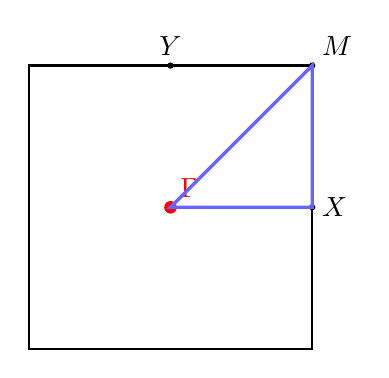
\begin{tikzpicture}[scale=1.0]
    \draw[thick] (-1.8,-1.8) rectangle (1.8,1.8);
    \fill[red] (0,0) circle (0.08) node[above right]{$\Gamma$};
    \fill (1.8,0) circle (0.04) node[right]{$X$};
    \fill (0,1.8) circle (0.04) node[above]{$Y$};
    \fill (1.8,1.8) circle (0.04) node[above right]{$M$};
    \draw[very thick,blue!60] (0,0)--(1.8,0)--(1.8,1.8)--cycle;
  \end{tikzpicture}
  \caption{方格晶格第一布里渊区与标准高对称点标注。常用路径为 $\Gamma\rightarrow X\rightarrow M\rightarrow\Gamma$。}
  \label{fig:bz-gamma}
\end{figure}

\section{从平面波展开理解能带为什么会出现}
如果把上一章的 Maxwell 方程和本章的 Bloch 形式合并起来，可以把周期介质中的模式进一步写成
\[
\E_{\kvec}(\rho,z)
=
\sum_{\gvec}\bm{c}_{\kvec+\gvec}(z)\,
\ee^{\ii(\kvec+\gvec)\cdot\rho}.
\]
这个展开式说明：在周期结构中，一个 Bloch 模并不是单一平面波，而是许多相差倒格矢的平面波分量的相干叠加。若没有周期调制，这些平面波彼此互不耦合；一旦周期调制存在，它们就通过介电函数的傅里叶分量彼此混合，于是原本简单的自由色散被“切开”和“重排”，这就是能带结构出现的根本原因。

对新手来说，这一步尤其关键。因为很多人第一次见到能带图时，会误以为它只是某种“把频率对波矢作图”的漂亮结果。实际上，能带是平面波在周期势中相互耦合后的本征值图谱。这个理解一旦建立，后面读到“带隙”“带折叠”“带边”“Gamma 点简并”时，就不再只是死记术语，而能回到“哪些平面波被耦合在一起”这个更基本的问题上。

\begin{ExampleBox}
对一维周期结构，最基本的带隙可以看成两个满足布拉格条件的反向平面波发生耦合后形成的分裂。二维 PCSEL 虽然复杂得多，但逻辑是一致的：只是参与耦合的波分量不再只有一对，而可能是一组等价方向的波。
\end{ExampleBox}

\section{二维光子晶体的常见晶格：方格与三角晶格}
PCSEL 文献中最常见的二维晶格是方格晶格和三角晶格。选择哪一种，不是审美问题，而会直接影响：
\begin{itemize}
  \item 高对称点的类型与简并结构；
  \item 等价散射方向的数量；
  \item 允许的偏振选择规则与远场工程路径。
\end{itemize}

方格晶格的优势是几何和对称性直观，很多最小耦合波图像都容易从这里建立；三角晶格则往往在六重对称条件下展现不同的模式简并与辐射特征。对初学者而言，先在方格晶格上建立直觉，再迁移到三角晶格，是比较稳妥的学习路径。

\subsection{三角晶格速览：后面为什么会频繁出现 \texorpdfstring{$K$}{K} 点与 \texorpdfstring{$C_{6v}$}{C6v}}
三角晶格的一个常用基矢选择是
\begin{equation}
\bm a_1 = a\hat{\bm x},
\qquad
\bm a_2 = a\left(\frac{1}{2}\hat{\bm x}+\frac{\sqrt{3}}{2}\hat{\bm y}\right).
\label{eq:triangular_real_basis}
\end{equation}
将它代入 \cref{eq:2d_reciprocal_general}，得到
\begin{equation}
\bm b_1 = \frac{2\pi}{a}\left(1,-\frac{1}{\sqrt{3}}\right),
\qquad
\bm b_2 = \frac{2\pi}{a}\left(0,\frac{2}{\sqrt{3}}\right).
\label{eq:triangular_reciprocal_basis}
\end{equation}
此时第一布里渊区是正六边形，最常见的高对称点是区中心 $\Gamma$、边中心 $M$ 和顶点 $K$。在标准笛卡尔坐标系下，这些点的坐标通常取为
\begin{equation}
\Gamma = (0,0),
\qquad
M = \left(\frac{\pi}{a},\frac{\pi}{\sqrt{3}a}\right),
\qquad
K = \left(\frac{4\pi}{3a},0\right).
\label{eq:triangular_high_symmetry_points}
\end{equation}
注意 $M$ 点是第一布里渊区六边形边的中点，而 $K$ 点是顶点。有时也会见到用倒格矢基底的约化坐标表示，例如 $K=(1/3,1/3)$，这取决于具体约定。这一节的任务不是立刻把三角晶格全部算透，而是给后文一个最小几何坐标系：当 \cref{ch:polarization,ch:bic} 讨论 $C_{6v}$ 小群、双重简并和六重对称散射时，读者至少知道这些标签对应的倒空间位置是什么。

\begin{figure}[htbp]
  \centering
  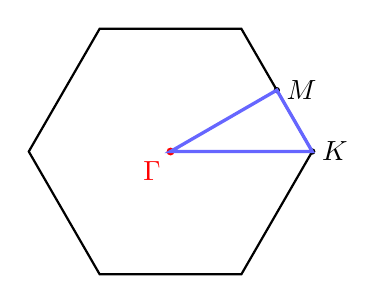
\begin{tikzpicture}[scale=1.0]
    \coordinate (G) at (0,0);
    \coordinate (K1) at (1.8,0);
    \coordinate (K2) at (0.9,1.5588);
    \coordinate (K3) at (-0.9,1.5588);
    \coordinate (K4) at (-1.8,0);
    \coordinate (K5) at (-0.9,-1.5588);
    \coordinate (K6) at (0.9,-1.5588);
    \draw[thick] (K1)--(K2)--(K3)--(K4)--(K5)--(K6)--cycle;
    \fill[red] (G) circle (0.05) node[below left]{$\Gamma$};
    \fill (1.8,0) circle (0.04) node[right]{$K$};
    \fill (1.35,0.7794) circle (0.04) node[right]{$M$};
    \draw[very thick,blue!60] (G)--(1.35,0.7794)--(1.8,0)--cycle;
  \end{tikzpicture}
  \caption{三角晶格第一布里渊区示意。最常用的高对称路径是 $\Gamma\rightarrow M\rightarrow K\rightarrow\Gamma$。}
  \label{fig:bz-triangular}
\end{figure}

\subsection{新手第一次看高对称路径时应看什么}
很多书或软件会直接给出一条高对称路径，比如方格晶格中的 $\Gamma\rightarrow X\rightarrow M\rightarrow\Gamma$。新手最容易犯的错误，是把注意力全部放在“哪条曲线高、哪条曲线低”，却忽略了真正更重要的问题：
\begin{enumerate}
  \item 哪些点是高对称点，为什么只看这些点；
  \item 某条带在这些点附近是否变平，意味着哪些耦合增强；
  \item 哪些带在高对称点重合，意味着可能存在简并与后续可控分裂。
\end{enumerate}
因此，第一次看高对称路径，不要急着评价“哪条带更好”，而要先学会读出“哪里在发生模式重组”。

\begin{ExampleBox}
若在方格晶格中只保留最主要的四个平面波分量，许多 $\Gamma$ 点耦合现象就能得到很清楚的图像。这也是为什么很多教材和早期解析模型喜欢从方格晶格开始，而不是一上来就讨论所有可能晶格。
\end{ExampleBox}

\section{把二维理想图像放回真实 PCSEL：slab 结构会带来什么变化}
到目前为止，我们讨论的 Bloch 理论主要是“平面内无限周期”的语言。但真实 PCSEL 不是严格二维材料，而是具有有限厚度的 slab 结构。也就是说，场不仅在平面内受周期调制，还在 $z$ 方向受外延层栈约束。这一事实会带来两个关键后果。

第一，真正的模式是全矢量三维模式。即使在某些参数区间内人们习惯说“TE-like”或“TM-like”，那也通常意味着“主要电场分量或主要磁场分量具有某种偏向”，而不是二维教科书中严格分离的纯 TE/TM 解。

第二，slab 的存在允许导模、泄露模和辐射模共存。某个在二维理想模型中看似被很好分类的 Bloch 模，放到有限厚度 slab 中以后，可能会通过垂直辐射通道与自由空间耦合，从而成为对 PCSEL 真正重要的候选模。

\begin{IntuitionBox}
二维 Bloch 理论的作用是告诉我们“平面内有哪些组织良好的模式家族”；slab 结构则提醒我们“这些家族在真实三维器件里会怎样与纵向约束和辐射通道重新混合”。PCSEL 正是在这两层之间工作。
\end{IntuitionBox}

\section{TE/TM 分类为什么常常只是近似}
在严格二维、无厚度、标量化处理的模型中，TE 与 TM 可以作为清晰的极化分类。但在真实 PCSEL slab 中，下列因素都会破坏这一理想图像：
\begin{itemize}
  \item 高折射率对比导致边界处矢量分量强烈耦合；
  \item 周期孔形和垂直不对称使场分量不再简单分离；
  \item 辐射通道要求场同时满足面内周期和垂直出射条件。
\end{itemize}

因此，后文若使用“TE-like”或“TM-like”这样的词，应理解为工程上的近似标签，而不是严格数学分类。本书采用一个可操作的判别标准：若模式电场能量中 $E_z$ 分量占比 $<5\%$，称为 \textbf{TE-like}；反之若 $H_z$ 分量占比 $<5\%$，称为 \textbf{TM-like}。这里的“like”提醒读者：只要 slab 上下不对称，$E_z$ 和 $H_z$ 都不可能严格为零，真实模式是混合极化的。这个提醒很重要，因为许多关于偏振和远场的误判，都源自把近似 TE/TM 标签当成了真实矢量模的完整描述。

\subsection{一个对初学者更安全的学习顺序}
如果读者刚接触 PCSEL，不必一上来就放弃所有 TE/TM 直觉。更安全的做法是分三步：
\begin{enumerate}
  \item 先用二维标量或 TE-like 图像理解带结构、带隙和高对称点；
  \item 再用全矢量 slab 模型检查哪些结论仍然成立，哪些开始偏移；
  \item 最后在有限尺寸和开放边界模型中验证偏振与远场。
\end{enumerate}
这种“先建立直觉，再主动拆掉过强近似”的路径，比一开始就把所有三维矢量细节压到新手身上更有效。

\begin{PitfallBox}
把二维平面波展开中的 TE/TM 标签直接搬到真实有限厚度电注入器件上，是 PCSEL 建模里非常常见的错误。尤其当外延不对称、金属邻近损耗或偏振工程很重要时，这种错误会直接影响模式判定。
\end{PitfallBox}
\begin{CommonPitfallBox}{把二维 TE/TM 当成三维 slab 的严格本征极化}
\textbf{常见误读：}在二维模型里标了 TE/TM，就直接把它当成真实器件中的“纯 TE/纯 TM 模”。

\textbf{正确做法：}把二维结果仅作为 TE-like/TM-like 的初筛标签，再用全矢量三维模型（含开放边界与有限尺寸）复核偏振、远场和阈值排序。

\textbf{典型后果：}
\begin{itemize}
  \item 把混合极化模误判为“纯偏振模”
  \item 误判法向辐射允许性与偏振选择规则
  \item 误把二维排序当成器件阈值排序
\end{itemize}
\end{CommonPitfallBox}

\section{Bloch 理论能告诉我们什么，又不能告诉我们什么}
到这一章结尾，必须把 Bloch 理论的能力边界说清楚。

它能告诉我们：
\begin{itemize}
  \item 周期结构中模式如何按 $\kvec$ 和对称性分类；
  \item 第一布里渊区内哪些高对称点值得重点关注；
  \item 某些简并与选择规则为何出现。
\end{itemize}

它不能单独告诉我们：
\begin{itemize}
  \item 有限器件边缘效应会不会改变模式排序；
  \item 有源区增益分布是否偏向目标模；
  \item 电注入和温升下哪一个模最终先起振并保持稳定。
\end{itemize}

因此，Bloch 理论是模式分类的起点，而不是 PCSEL 器件结论的终点。

\section{通向下一章：为什么 Gamma 点会成为中心舞台}
本章已经说明：二维周期结构中的模式可以用 Bloch 波矢分类，而 $\Gamma$ 点是布里渊区中心的特殊位置。下一章将进一步回答：为什么在 PCSEL 中，$\Gamma$ 点附近的模式经常成为重点关注对象？简并、对称性、辐射耦合和有限尺寸修正又会怎样共同决定真正的候选激射模？

\section*{本章小结}
Bloch 定理把无限周期结构的求解组织成了按波矢分类的问题，并由此引出倒格矢、布里渊区和高对称点等核心概念。对 PCSEL 而言，这一步的意义在于建立候选模的“目录系统”。但这还只是目录，目录之后还要讨论哪些模式真正与辐射、增益和器件工作条件相匹配。

\section*{练习题}
\begin{enumerate}
  \item \basicq 从平移算符的角度，重述一次 Bloch 定理的证明思路。

  \item \basicq 证明 $\kvec$ 与 $\kvec+\gvec$ 对应相同的 Bloch 相位条件。

  \item \midq 解释为什么 $\Gamma$ 点的重要性不仅仅来自“群速度小”，还来自模式对称性和辐射通道。

  \item \hardq 给出一个 slab 结构中 TE/TM 近似可能失效的具体场景。
\end{enumerate}

\section*{建议继续阅读}
\begin{itemize}
  \item \cite{joannopoulos2008,sakoda2005} 中关于 Bloch 定理与二维光子晶体的基础章节。 这条阅读的重点是补足本章关于Bloch 定理、布里渊区与模式分类 的标准背景、经典语言和代表性文献接口。

  \item 读完下一章后再回看本章，通常会更容易理解 $\Gamma$ 点为何成为 PCSEL 模选择的核心位置。 这条阅读的重点是把本章的输出顺着主线接到后续模块，而不是停成孤立知识点。
\end{itemize}

